\documentclass[]{article}

\usepackage{lmodern}
\usepackage{amssymb,amsmath}
\usepackage{ifxetex,ifluatex}

\usepackage[a4paper, left=2cm, right=2cm, top=2cm]{geometry} % Breite der Seitenränder

\usepackage{listings} % code

%\usepackage{pdflscape} % Landscape mode
\usepackage{lscape} % Landscape mode

\usepackage[ngerman]{babel} % German language
\usepackage[normalem]{ulem} % Strikethrough
\usepackage{titlesec}
\newcommand{\sectionbreak}{\clearpage} % Neues Seite nach Section
\usepackage{enumitem} % Liste mit description

%\usepackage{fixltx2e} % provides \textsubscript
\ifnum 0\ifxetex 1\fi\ifluatex 1\fi=0 % if pdftex
  \usepackage[T1]{fontenc}
  \usepackage[utf8]{inputenc}
\else % if luatex or xelatex
  \ifxetex
    \usepackage{mathspec}
  \else
    \usepackage{fontspec}
  \fi
  \defaultfontfeatures{Ligatures=TeX,Scale=MatchLowercase}
\fi
% use upquote if available, for straight quotes in verbatim environments
\IfFileExists{upquote.sty}{\usepackage{upquote}}{}
% use microtype if available
\IfFileExists{microtype.sty}{%
\usepackage{microtype}
\UseMicrotypeSet[protrusion]{basicmath} % disable protrusion for tt fonts
}{}
\usepackage[unicode=true]{hyperref}
\hypersetup{
            pdftitle={arc42 Template},
            pdfborder={0 0 0},
            breaklinks=true}
\urlstyle{same}  % don't use monospace font for urls
\usepackage{longtable,booktabs}
\usepackage{tabularx}
% Fix footnotes in tables (requires footnote package)
\IfFileExists{footnote.sty}{\usepackage{footnote}\makesavenoteenv{long table}}{}
\usepackage{graphicx,grffile}
\makeatletter
\def\maxwidth{\ifdim\Gin@nat@width>\linewidth\linewidth\else\Gin@nat@width\fi}
\def\maxheight{\ifdim\Gin@nat@height>\textheight\textheight\else\Gin@nat@height\fi}
\makeatother
% Scale images if necessary, so that they will not overflow the page
% margins by default, and it is still possible to overwrite the defaults
% using explicit options in \includegraphics[width, height, ...]{}
\setkeys{Gin}{width=\maxwidth,height=\maxheight,keepaspectratio}
\IfFileExists{parskip.sty}{%
\usepackage{parskip}
}{% else
\setlength{\parindent}{0pt}
\setlength{\parskip}{6pt plus 2pt minus 1pt}
}
\setlength{\emergencystretch}{3em}  % prevent overfull lines
\providecommand{\tightlist}{%
  \setlength{\itemsep}{0pt}\setlength{\parskip}{0pt}}
\setcounter{secnumdepth}{0}
% Redefines (sub)paragraphs to behave more like sections
\ifx\paragraph\undefined\else
\let\oldparagraph\paragraph
\renewcommand{\paragraph}[1]{\oldparagraph{#1}\mbox{}}
\fi
\ifx\subparagraph\undefined\else
\let\oldsubparagraph\subparagraph
\renewcommand{\subparagraph}[1]{\oldsubparagraph{#1}\mbox{}}
\fi

% set default figure placement to htbp
\makeatletter
\def\fps@figure{htbp}
\makeatother


\title{
\includegraphics{images/arc42-logo.png} Template}
\date{\today}
\author{Christoph Hellmich}

\begin{document}

\maketitle
\thispagestyle{empty} % Don't show page number on title page

\tableofcontents

\section*{}

\textbf{Über arc42}

arc42, das Template zur Dokumentation von Software- und
Systemarchitekturen.

Erstellt von Dr. Gernot Starke, Dr. Peter Hruschka und Mitwirkenden.

Template Revision: 7.0 DE (asciidoc-based), January 2017

© We acknowledge that this document uses material from the arc 42
architecture template, \url{http://www.arc42.de}. Created by Dr. Peter
Hruschka \& Dr. Gernot Starke.

\section{Einführung und Ziele}\label{section-introduction-and-goals}

Dieses Dokument beschreibt die Softwarearchitektur des AutoLiefer-Systems für das automatische Erfassen und Verarbeiten von Lieferscheinen für das Unternehmen CarLogistic AG.

\paragraph{Vision der FA. CarLogistic AG}

Optimierung der Prozesse für die Buchhaltung, um langfristig die Qualität der Verwaltung zu garantieren (Agenda bis 2025).

\paragraph{Geschäftsziele}

\begin{description}
  \item [Z1] Steigerung der Effektivität bei der Überprüfung eingegangener Lieferscheine und Rechnungen durch die Senkung von manuellen Schritten sowie der Erhöhung der Teilautomatisierung. Erhoffte Vorteile:
  \begin{itemize}
    \item Senkung der Fehlerquote bei der Überprüfung von Lieferscheinen und Rechnungen
    \item Generelle Entlastung der zuständigen Mitarbeiter
    \item Skalierbarer Ansatz für die Zukunft
  \end{itemize}
  \item [Z2] Integration von Techniken zur Auswertung und Bewertung von Vorgängen, die zu einer kontinuierlichen Optimierung des Prozesses führen.
  \item [Z3] Erhöhte Anpassbarkeit der Prozesse für zukünftige Anforderungen
\end{description}

\paragraph{Ausgangssituation}

Abbildung \ref{fig:01_Ist-Situation-Kontext} zeigt die Ist-Situation bei Projektbeginn als Paketdiagramm.

\begin{figure}
  \centering
  \includegraphics{images/01_Ist-Situation-Kontext.png}
  \caption{Ist-Situation}
  \label{fig:01_Ist-Situation-Kontext}
\end{figure}

Die in Abbildung \ref{fig:01_Ist-Situation-Kontext} dargestellten Systeme sind in Tabelle \ref{tab:Ist-Situation-Systeme} beschrieben.

\begin{table}[b]
\centering
\caption{Ist-Situation Systeme}
\label{tab:Ist-Situation-Systeme}
\begin{tabularx}{\linewidth}{@{}llX@{}}
\toprule
System          & Art                  & Beschreibung \\
\midrule
HWeis 1.0       & Überweisungssoftware & Rechnnungen überweisen \\
Openbravo       & ERP-System           & Posten und Betrag der Rechnung eintragen \\
MyOpenbravoTool & Desktop-Anwendung    & Client-Tool für den Zugriff auf Openbravo \\
Siebel          & CRM-System           & Speicherung von Stammdaten und beweglichen Daten \\
Novis           & CRM-System           & Speicherung von Stammdaten und beweglichen Daten \\
\bottomrule
\end{tabularx}
\end{table}


 In Abbildung \ref{fig:02_Ist-Szenario-Verlauf} ist ein möglicher Ablauf dargestellt, der bei einer Annahme einer Bestellung durchlaufen wurde.

\begin{figure}
  \centering
  \includegraphics{images/02_Ist-Szenario-Verlauf.png}
  \caption{Aktuelles (As-Is) Szenario zur Orientierung (Standard Verlauf)}
  \label{fig:02_Ist-Szenario-Verlauf}
\end{figure}

\subsection{Aufgabenstellung}\label{_aufgabenstellung}

Anforderungen, die im Prototypen implementiert wurden, sind nachfolgend \textbf{fett} hervorgehoben. Auslassungen gegenüber den ursprünglichen Anforderungen sind \sout{durchgestrichen} und Hinzufügungen stehen in [eckigen] Klammern. Anschließend sind in Abbildung \ref{fig:03_Use-Case_Ausschnitt} die Anforderungen in einem Use-Case-Diagramm zusammengefasst.

\paragraph{Funktionale Anforderungen (Sicht Auftraggeber = Mitarbeiter der CarLogistic)}

\begin{description}
  \item[FA1] Der Auftraggeber der Bestellung (Mitarbeiter der CarLogistic) soll in der Lage sein, Lieferscheine einscannen zu können.
  \item[FA2] \textbf{Der Auftraggeber der Bestellung muss in der Lage sein, die wichtigsten Daten eines Lieferscheines manuell in einer Eingabemaske einzugeben}, falls kein Scanner vorhanden ist.
  \item[FA3] \textbf{Der Auftraggeber der Bestellung sollte in der Lage sein,} einen eingescannten Lieferschein oder \textbf{einen manuell erfassten Lieferschein mit einer Anmerkung zu annotieren.}
  \item[FA4] Der Auftraggeber der Bestellung sollte in der Lage sein, einen eingescannten Lieferschein oder einen manuell erfassten Lieferschein mittels digitaler Signatur zu unterschreiben.
  \item[FA5] \textbf{Die digital erfassten Lieferscheine müssen persistent in einem ECM gespeichert werden. Der importierte Lieferschein sollte dabei in einem gängigen Format abgespeichert werden. Das ECM befindet sich in der Abteilung Controlling.}
  \item[FA6] \sout{Die persistent abgespeicherten Lieferscheine müssen für spätere Bearbeitungen abrufbar sein.} [Redudant FA9]
  \item[FA7] \textbf{Der Auftraggeber der Bestellung muss in der Lage sein, den} eingescannten oder \textbf{manuell eingegebenen Lieferschein an die Buchhaltung der CarLogistic abzuschicken.}
  \item[FA8] Der Auftraggeber der Bestellung kann über den Status bei der weiteren Bearbeitung (z.B. Eskalation) durch das System stets unterrichtet werden. Dazu steht dem Auftraggeber eine entsprechende Web-Schnittstelle zur Verfügung.
  \item[FA9] \textbf{Der Auftraggeber soll in der Lage sein, von Seiten der Buchhaltung der CarLogistic als falsch deklarierte Lieferscheine wieder zu empfangen und diese ggf. gemäß den Anmerkungen der Buchhaltung zu überarbeiten.}
  \item[FA10] Der Auftraggeber kann sich Statistiken über seine abgeschlossenen Vorträge anzeigen lassen.
\end{description}

\paragraph{Funktionale Anforderungen (Sicht Mitarbeiter Buchhaltung der CarLogistic)}

\begin{description}
  \item[FA11] Der Rechnungsempfänger (ein ungeschulter Mitarbeiter Buchhaltung der CarLogistics, typischerweise eine studentische Hilfskraft) soll in der Lage sein, per Post eingegangene Rechnungen von Lieferanten einscannen zu können.
  \item[FA12] \textbf{Die importierte Rechnung pro Lieferant sollte in einem gängigen Format in einem ECM archiviert werden.}
  \item[FA13] \textbf{Der Rechnungsempfänger muss in der Lage sein, die wichtigsten Daten einer Rechnung manuell einzugeben}, falls kein Scanner vorhanden ist.
  \item[FA14] Der Rechnungsempfänger muss in der Lage sein, elektronisch eingegangene Rechnungen vom Lieferanten zu empfangen und über dieses Ereignis entsprechend unterrichtet zu werden.
  \item[FA15] \textbf{Der Rechnungsempfänger sollte in der Lage sein, eine} eingescannte, \textbf{manuell erfasste} oder elektronisch empfangene \textbf{Rechnung mit einer Anmerkung zu annotieren.}
  \item[FA16] \textbf{Der Rechnungsempfänger muss in der Lage sein, eine} eingescannte, \textbf{manuell erfasste} oder elektronisch empfangene \textbf{Rechnung zur weiteren Bearbeitung an den Rechnungsprüfer weiterzuschicken.}
  \item[FA17] \sout{Der Rechnungsempfänger möchte die Eskalation von Rechnungen und Lieferscheinen vornehmen (inkl. Kommentar). Der Einkäufer wird dabei in bestimmten Fällen unmittelbar unterrichtet, um die Reaktionszeit auf stark eskalierte Vorgänge zu reduzieren. Eine Eskalation erfolgt bei einfachen bis zu gravierenden Abweichungen in der Lieferung und der Rechnungsstellung. Eine Eskalation hängt auch von dem betreffenden Unternehmen ab sowie von der Anzahl vergangener Eskalationen.} [Widerspruch FA27]
  \item[FA18] \sout{Für Statistikzwecke müssen die eingegangen Rechnungen pro Lieferant persistent gespeichert werden.} [Redudant FA12] \sout{Zudem müssen die importierten Lieferscheine der Auftraggeber persistent gespeichert werden. Der importierte Lieferschein sollte dabei in einem gängigen Format abgespeichert werden.}[Redudant FA5] \sout{Hierzu sollte das ECM der Abteilung Marketing verwendet werden.} [Widerspruch FA5]
   \item[FA19] \textbf{Der Rechnungsprüfer (Mitarbeiter in der Buchhaltung der CarLogistic, typischerweise ein erfahrener Buchalter mit mehrjähriger Erfahrung) wird vom System regelmäßig über eingehende Lieferscheine (von Seiten des Auftraggebers)} \sout{unterrichtet (Email-Notifikation oder Signal in der Client-Applikation)}\textbf{, [mittels eines neuen Eintrags in seiner personalisierten Task-Liste innerhalb der Client-Anwendung unterrichtet, vgl. FA20 und FA21.]}
  \item[FA20] \textbf{Der Rechnungsprüfer wird vom System regelmäßig über eingehende Rechnungen unterrichtet. Dazu erhält der Rechnungsprüfer entsprechend einen neuen Eintrag in seiner personalisierten Task-Liste innerhalb der Client-Anwendung.}
  \item[FA21] \textbf{Das System soll \sout{identische} [zusammengehörige] Rechnungen und Lieferscheine identifizieren und ein Zusammenhang dem Rechnungsprüfer vorschlagen und in seiner personalisierten Task-­Liste ablegen.} \sout{Eine Bestätigung des Zusammenhangs} \textbf{[Die Zuordnung des Systems] muss der Rechnungsprüfer bestätigen.}
  \item[FA22] Der Rechnungsprüfer soll in der Lage sein, Bezüge zwischen Rechnungen und Lieferscheinen manuell herzustellen, falls das System keine Bezüge hat herstellen können.
  \item[FA23] \textbf{Falls der Lieferschein[, dem eine Rechnung zugewiesen wurde,] eine Lieferung bestätigt, so kann die Bearbeitung des Rechnungsbetrags durchgeführt werden. Diese Bestätigung wird in dem Vorgang persistent gespeichert (Datum, Kommentar usw.)}
  \item[FA24] \textbf{Die Banküberweisung des Rechnungsbetrags an die Bank wird automatisiert durch das System ausgelöst.}
  \item[FA25] \textbf{Die Buchung des Rechnungsbetrags in die Finanzbuchhaltung des ERP-­Systems soll automatisiert durch das System erfolgen.}
  \item[FA26] Kann die Überweisung wegen einer fehlerhaften Lieferung nicht ausgeführt werden, so ist die Rechnung dem Lieferanten digital oder per Post zurückzuschicken. Der Vermerk des Mitarbeiters aus dem Lieferschein soll dabei verlustfrei übernommen werden. Diese Ablehnung wird in dem Vorgang persistent gespeichert (Datum, Kommentar).
  \item[FA27] \textbf{Der Rechnungsprüfer muss die Eskalation von Rechnungen und Lieferscheinen initiieren können. Bei einer Eskalation soll er zunächst einen erklärenden Kommentar eingeben. Der Einkäufer, in kritische Fällen aber auch andere Stakeholder (z.B. Einkäufer, Vorstand, Präsident) werden dabei in bestimmten Fällen unmittelbar anhand verschiedener Eskalationsstufen unterrichtet, um die Reaktionszeit auf stark eskalierte Vorgänge zu reduzieren. Nur der Rechnungsprüfer darf Eskalationen vornehmen.}
  \begin{description}
    \item[Stufe 1] Differenz Rechnung und Lieferschein < 100: Einkäufer informieren
    \item[Stufe 2] Differenz Rechnung und Lieferschein zwischen 100 und 1000: Vorstand informieren
    \item[Stufe 3] Differenz Rechnung und Lieferschein > 1000: Präsident informieren
  \end{description}
  \item[FA28] \textbf{Der Rechnungsprüfer kann nicht korrekt ausgefüllte Lieferscheine an den Auftraggeber zurücksenden, mit der Bitte um Überarbeitung (inkl. Kommentar).}
  \item[FA29] Bei der Kontrolle von stark abweichenden Rechnungen und Lieferscheinen (gemäß Eskalationsstufen) gilt das Vier­‐Augen­‐Prinzip.
  \item[FA30] Bei vertrauenswürdigen Lieferanten kann der Prozess (Abgleich elektronisch eingegangene Rechnung mit Lieferschein, Verbuchung, Überweisung, Archivierung) automatisiert ablaufen.
\end{description}

\paragraph{Funktionale Anforderungen (Einkäufer der CarLogistic)}

Anmerkung: der Einkäufer ist eine Rolle in der Verwaltung, der für den Einkauf sämtlicher Güter und Dienstleistungen zuständig ist.

\begin{description}
  \item[FA31] Der Einkäufer des Unternehmens soll über ein Cockpit die fachliche Leistungsfähigkeit des neuen Prozesses mit Hilfe von Key Performance Indicators (KPI) regelmäßig unterrichtet werden.
  \begin{description}
    \item[KPI1] Wie oft werden Rechnungen an einen Lieferer zurückgeschickt?
    \item[KPI2] Wie oft wird von welchem Lieferer bestellt?
    \item[KPI3] Wie oft hat das System automatisch und korrekt einen Bezug zwischen Lieferschein und Rechnung hergestellt?
    \item[KPI4] Wie oft hat das System einen falschen Bezug zwischen Lieferschein und Rechnung hergestellt?
    \item[KPI5] Wie oft wurde welche Eskalationsstufe erreicht?
  \end{description}
  \item[FA32] Der Einkäufer soll über alle abgeschlossenen Vorgänge (definiert von der eigentlichen Bestellung bis zur Rechnungsüberweisung) wöchentlich vom System in Form eines Reports unterrichtet werden.
  \item[FA33] \textbf{Der Einkäufer nimmt Eskalationen von Seiten der Rechnungsprüfung täglich in Form eines Reports entgegen. Der Einkäufer kommentiert diese (Kommentar wird zum Vorgang gespeichert) und entscheidet ad hoc über den weiteren Vorgang (→ separater Fall mit verschiedenen Handlungsoptionen, die er situativ auswählen kann). Eine Eskalation wird nur intern verarbeitet, eine Weiterleitung an den Lieferanten ist nicht vorgesehen.}
\end{description}

\paragraph{Funktionale Anforderungen (Lieferant)}

\begin{description}
  \item[FA34] Der Lieferant soll über eine Schnittstelle, elektronische Rechnungen an die CarLogistics versenden können. Die Erstellung der Rechnung soll nicht Bestandteil des Systems sein.
  \item[FA35] \sout{Zur Förderung der besseren Zusammenarbeit und Zuverlässigkeit möchte der Lieferant bei hoch eingestuften Eskalationen unmittelbar vom System unterrichtet werden.} [Widerspruch FA33]
\end{description}

\paragraph{Technische Anforderungen (gestellt von der IT-Abteilung)}

\begin{description}
  \item[TA1] Die technische Abteilung wünscht sich eine zentrale Kommunikation über eine Komponente, um die Kommunikation in der Software-Architektur besser überwachen und loggen zu können. Der technischen Abteilung ist die Komplexität einer solchen Lösung durchaus bewusst und möchte eine Einschätzung hinsichtlich der Machbarkeit / Rentabilität haben. [ESB]
  \item[TA2] Die technische Abteilung möchte eine zentrale Registry zur Verwaltung der implementierten Services haben. [Service Registry]
  \item[TA3] \textbf{Die technische Abteilung wünscht sich, auch in fachlicher Abstimmung mit dem Einkäufer, eine flexible Art und Weise, um Eskalationsregeln ändern zu können. Auch über die Darstellung von Eskalationsregeln möchte die technische Abteilung eine Information haben.} [BRE]
  \item[TA4] Die technische Abteilung soll über ein Cockpit die technische Leistungsfähigkeit des neuen Prozesses mit Hilfe von Key Performance Indicators (KPI) regelmäßig unterrichtet werden. [BAM]
  \item[TA5] \textbf{Die technische Abteilung soll in der Lage sein, wichtige Abläufe in der Architektur als Workflow zu ändern und in der Umgebung einzusetzen. Damit sollen zudem auch zukünftig neue Geschäftsprozesse flexibel und agil unterstützt werden.} [BPM/BPMN]
  \item[TA6] \textbf{Die technische Abteilung wünscht sich nachvollziehbare Abkommen zwischen den Lieferanten, der CarLogistics, um etwaige Datenvolumen, Zugriffe auf Systeme zu regulieren. Diese Abkommen sollen auf belastbaren Annahmen basieren.} [SLA]
  \item[TA7] \textbf{Die technische Abteilung wünscht sich einen State-Of-The-Art Ansatz zur Entwicklung der notwendigen Client-Anwendung inklusive der Umsetzung von personalisierten Task-Listen. Die Anwendung sollte möglichst einheitlich sein, um ein Corporate Design zu realisieren.} [Web-User-Interface]
  \item[TA8] Die technische Abteilung möchte eine technische Unterstützung haben zur Umsetzung der Eskalation seitens des Einkäufers (FA33). Er möchte einen State of the Art Ansatz haben, wie man ad hoc ausführbare Handlungsoptionen modellieren und implementieren kann. [BPM/CMMN]
  \item[TA9] \textbf{Die technische Abteilung möchte zur Kostenreduktion wichtige Bestandteile der Architektur in eine Cloud auslagern und ist hierzu auch gerne an Lösungsstrategien interessiert.} [\textbf{On-Premise} vs. Cloud]
  \item[TA10] \textbf{Die technische Abteilung möchte generell die Skalierbarkeit sowie die Ausfallsicherheit der Gesamt-Architektur optimieren, damit auch in Zukunft mit einer steigenden Anzahl von Benutzern und Daten umgegangen werden kann.} [Skalierbarkeit und Ausfallsicherheit, nur modellieren]
\end{description}

\paragraph{Forschungsperspektiven (Prof. Mayer, Leiter Innovationsabteilung)}

\begin{description}
  \item[FF1] \textbf{Ein Professor wünscht sich ein Modell zur Empfehlung einer Handlungsoption, die dem Einkäufer die bestmögliche Variante präsentiert, die er dann auswählen kann (betr. FA33). Eine prototypische Implementierung wäre auch wünschenswert.}
\end{description}

\begin{figure}
  \centering
  \includegraphics{images/03_Use-Case_komplett.png}
  \caption{Use-Case-Diagramm}
  \label{fig:03_Use-Case_Ausschnitt}
\end{figure}

\subsection{Qualitätsziele}\label{_qualitaetsziele}

Das primäre Qualitätsziel für das vorliegende Projekt ergibt sich aus der technischen Anforderung 3 (TA3). Die Eskalationsregeln sollen komfortabel bearbeitet werden können. Für die Verwaltung der Eskalationsregeln wird eine Business Rules Engine (BRE) verwendet.

Des Weiteren soll das System nach der technischen Anforderung 10 (TA10) skalierbar sein.

Weitere Qualitätsziele für die Entwicklung des Prototypen sind:
\begin{description}
  \item[Verständlichkeit] Der Code soll einfach zu verstehen und der Lösungsweg leicht zu adaptieren sein.
  \item[Funktionalität] Der Prototyp soll eine möglichst hohe Zahl der Anforderungen erfüllen.
  \item[Änderbarkeit] Es sollten nur die nötigsten Entwurfsentscheidungen getroffen werden. Zwischen einzelnen Entscheidungen sollte möglichst keine Abhängigkeit bestehen.
  \item[Anpassbarkeit] Der Prototyp sollte offen für Ergänzungen und Erweiterungen sein. Eine hohe Testabdeckung könnte dies beispielsweise erschweren.
\end{description}

\subsection{Stakeholder}\label{_stakeholder}

Die Tabelle \ref{tab:Stakeholder} zeigt die konkreten Stakeholder für das System sowie deren Erwartungshaltung.

\begin{table}[bh]
\centering
\caption{Stakeholder}
\label{tab:Stakeholder}
\begin{longtable}[]{@{}lll@{}}
\toprule
\begin{minipage}[b]{0.19\columnwidth}\raggedright\strut
Rolle\strut
\end{minipage} & \begin{minipage}[b]{0.27\columnwidth}\raggedright\strut
Beschreibung\strut
\end{minipage} & \begin{minipage}[b]{0.46\columnwidth}\raggedright\strut
Erwartungshaltung\strut
\end{minipage}\tabularnewline
\midrule
\endhead
\begin{minipage}[t]{0.19\columnwidth}\raggedright\strut
Auftraggeber\strut
\end{minipage} & \begin{minipage}[t]{0.27\columnwidth}\raggedright\strut
Mitarbeiter der CarLogistic; erhält Lieferschein\strut
\end{minipage} & \begin{minipage}[t]{0.46\columnwidth}\raggedright\strut
Entlastung\strut
\end{minipage}\tabularnewline
\begin{minipage}[t]{0.19\columnwidth}\raggedright\strut
Rechnungsempfänger\strut
\end{minipage} & \begin{minipage}[t]{0.27\columnwidth}\raggedright\strut
Mitarbeiter aus der Buchhaltung; erhält Rechung\strut
\end{minipage} & \begin{minipage}[t]{0.46\columnwidth}\raggedright\strut
Unterstützung bei der Einpflege von Rechnungen in das System\strut
\end{minipage}\tabularnewline
\begin{minipage}[t]{0.19\columnwidth}\raggedright\strut
Rechnungsprüfer\strut
\end{minipage} & \begin{minipage}[t]{0.27\columnwidth}\raggedright\strut
Mitarbeiter aus der Buchhaltung; verarbeitet Rechung und Lieferschein\strut
\end{minipage} & \begin{minipage}[t]{0.46\columnwidth}\raggedright\strut
Ünterstützung bei der Zuordnung von Lieferscheinen und Bestellungen\strut
\end{minipage}\tabularnewline
\begin{minipage}[t]{0.19\columnwidth}\raggedright\strut
Einkäufer\strut
\end{minipage} & \begin{minipage}[t]{0.27\columnwidth}\raggedright\strut
Mitarbeiter aus der Verwaltung; überwacht Bestellung\strut
\end{minipage} & \begin{minipage}[t]{0.46\columnwidth}\raggedright\strut
Benachrichtigung, sobald Probleme mit einer Bestellung auftreten; Überblick über getätigte Bestellungen.\strut
\end{minipage}\tabularnewline
\begin{minipage}[t]{0.19\columnwidth}\raggedright\strut
IT-Abteilung\strut
\end{minipage} & \begin{minipage}[t]{0.27\columnwidth}\raggedright\strut
Wartet das zu entwickelnde System\strut
\end{minipage} & \begin{minipage}[t]{0.46\columnwidth}\raggedright\strut
Leichte Anpassbarkeit und Überwachung des Geschäftsprozesses\strut
\end{minipage}\tabularnewline
\begin{minipage}[t]{0.19\columnwidth}\raggedright\strut
Lieferant\strut
\end{minipage} & \begin{minipage}[t]{0.27\columnwidth}\raggedright\strut
Bringt die Bestellung zum Auftraggeber in die CarLogistic\strut
\end{minipage} & \begin{minipage}[t]{0.46\columnwidth}\raggedright\strut
Schnelle Bezahlung des Rechungsbetrags\strut
\end{minipage}\tabularnewline
\begin{minipage}[t]{0.19\columnwidth}\raggedright\strut
Prof. Mayer\strut
\end{minipage} & \begin{minipage}[t]{0.27\columnwidth}\raggedright\strut
Leiter der Innovationsabteilung\strut
\end{minipage} & \begin{minipage}[t]{0.46\columnwidth}\raggedright\strut
Erkenntnisgewinn\strut
\end{minipage}\tabularnewline
\bottomrule
\end{longtable}
\end{table}


\section{Randbedingungen}\label{section-architecture-constraints}

In diesem Abschnitt sind die Randbedingungen für das AutoLiefer-System beschrieben.

\subsection{Technische Randbedingungen}

Betrieb der Lösung auf einem marktüblichen Standard-Notebook, um sie im Rahmen einer Präsentation oder evtl. als Referenz (Bewerbungen etc.) auf einem solchen vorstellen bzw. besprechen zu können.

Für die Ausführung der Anwendung wird Java ab Version 8 und ein Web-Browser benötigt. Die Anwendung kann von der Kommandozeile aus gestartet werden.

Für das Projekt steht kein Budget zur Verfügung. Es können nur kostenlose Bibliotheken und Services verwendet werden.

\subsection{Organisatorische Randbedingungen}

Folgende Service Level Agreements sind einzuhalten:
\begin{description}
  \item[SLA1] Rechnungen dürfen eine Größe von 12 MB nicht überschreiten.
  \item[SLA2] Alle eingehenden Rechnungen werden innerhalb von 7 Tagen verarbeitet.
  \item[SLA3] Der Service, um Rechnungen zu übertragen, steht 24 Stunden am Tag, 7 Tage die Woche mit einer Ausfallrate von maximal 0,1\% im Jahr zur Verfügung.
\end{description}

Des Weiteren soll der Prototyp bis zum 12. September fertiggestellt werden. Die Dokumentation soll bis zum 16. September den finalen Zustand erreichen.

\section{Kontext}\label{section-system-scope-and-context}

\subsection{Fachlicher Kontext}

\begin{figure}
  \centering
  \includegraphics{images/Fachlicher_Kontext.png}
  \caption{Fachlicher Kontext}
  \label{fig:Fachlicher_Kontext}
\end{figure}

\paragraph{Anwender}

Anwender des Systems AutoLiefer sind Auftraggeber, Rechnungsprüfer, Rechnungsempfänger, Einkäufer und Lieferant, vgl. Stakeholder.

\paragraph{Lieferschein}

Der Lieferschein wird vom Auftraggeber entgegengenommen, unterschrieben und in das System eingepflegt. Der Rechnungsprüfer bzw. das System versucht, zu jedem Lieferschein die zugehörige Rechnung zu finden. Stellt der Rechnungsprüfer Fehler hinsichtlich des Lieferscheins fest, wird dieser inklusive Kommentar, seitens des Rechnungsprüfers, an den Auftraggeber zur Korrektur zurückgesendet.

\paragraph{Rechnung}

Eine Rechnung wird vom Lieferanten ausgestellt. Der Rechnungsprüfer erhält die Rechnung und pflegt diese, ggf. mit einem Kommentar, in das System ein. Der Rechnungsprüfer kontrolliert die Rechnung. Falls bei der Prüfung Mängel festgestellt wurden, wird die Rechnung inklusive eines Kommentars an den Lieferanten gesendet. Andernfalls, bei einer erfolgreichen Prüfung, wird eine Banküberweisung ausgeführt.

\paragraph{Eskalationen}

Der Rechnungsprüfer initiiert Eskalationen von Rechnungen und Lieferscheinen. Eine Eskalation erfolgt bei einfachen bis zu gravierenden Abweichungen in der Lieferung und der Rechnungsstellung.

\subsection{Technische Kontext}

In Abbildung \ref{fig:Technischer_Kontext} ist der technische Kontext des AutoLiefer-Systems beschrieben.

\begin{figure}
  \centering
  \includegraphics{images/Technischer_Kontext.png}
  \caption{Technisher Kontext}
  \label{fig:Technischer_Kontext}
\end{figure}

\paragraph{ERP-System: OpenBravo}

Der eingegangene Posten und der Betrag der überwiesenen Rechnung wird in der Finanzbuchhaltung eingetragen. Dies erfolgt manuell in dem ERP-System Openbravo. % FA25

\paragraph{Überweisungs-System: HWeis 1.0}

Falls der Lieferschein den ordnungsgemäßen Empfang der Ware bestätigt, wird die Überweisung der Rechnung beantragt. Diese Überweisung erfolgt manuell über eine eigen entwickelte Überweisungssoftware (HWeis 1.0), einer internen Web-Anwendung, welche als Webserver (Tomcat 7) bereitgestellt wird.

Der Aufruf von HWeis erfolgt über Java Servlet-Schnittstelle. Es werden sowohl Anfragen mittels GET als auch POST unterstützt, um Rechnungen zu überweisen, zu speichern und zu löschen. Außerdem können Reports für die Quartalsabrechnung erzeugt, Stammdaten der Mitarbeiter verifiziert und die Raumplanung der Mitarbeiter vorgenommen werden.

Falls eine Rechnung überwiesen wurde, dann erfolgt ein Signal via RMI (an die Client-Anwendung MyOpenbravoTools), dass die Rechnung verbucht werden konnte. Im Fall einer Verbuchung, erfolgt ein Signal von OpenBravo zurück zu HWeis 1.0 zur „Fertigstellung des Vorgangs“.

\paragraph{CRM-Systeme: Novis und Siebel}

Stammdaten und bewegliche Daten werden in zwei verschiedenen CRM-Systemen (Siebel und die Eigenentwicklung „Novis“) festgehalten, die vom Bereich CRM betrieben werden. Beide CRM-Systeme werden von OpenBravo und HWeis verwendet. Beide CRM-Systeme sind stets vom Datenbestand her konsistent abgeglichen. Dies wird durch eine PHP-Skript (abgeschlossene Bachelor Thesis im FB Informatik) innerhalb der Software Novis realisiert, die wöchentlich die Daten zwischen den CRMs abgleicht.

\paragraph{ECM-System}

In dem ECM-System werden Lieferscheine und Rechnungen gespeichert. %FA5, FA18

\section{Lösungsstrategie}\label{section-solution-strategy}

Für die Entwicklung des Prototypen liegt der Fokus auf der Verwendung von Funktionalität bestehender Lösungen, um von Best Practice erfahrener Entwickler profitieren zu können. Anschließend wird situativ entschieden, wo die Entwicklung eigener Funktionalität nötig ist.

Die Camunda Plattform enthält viele Funktionen, die für die Umsetzung der Anforderungen des AutoLiefer-Sytems aufgegriffen werden können. Die Modellierung der Workflows und der Entscheidungstabellen erfolgt mit dem Camunda Modeler, so dass die Bearbeitung von Abläufen bzw. der Regeln auch ohne Programmierkenntnisse möglich sind. Die Steuerung der Workflows und die Auswertung der Entscheidungstabellen übernimmt die Camunda Workflow Engine bzw. Camunda Decision Engine. Die Anzeige und Bearbeitung von Tasks wird mit der Camunda Taskslist realisiert, um zu vermeiden, eigenständig eine Benutzerverwaltung für den Prototypen implementiert zu müssen. Der Status der Workflows kann mit dem Camunda Cockpit abgerufen werden. Reports müssen selber erstellt werden, da die Funktionen nur in der kostenpflichtigen Enterprise Version von Camunda angeboten wird.

Die Benutzerfreundlichkeit und Fehlerbehandlung hat für die Umsetzung des Prototypen niedrige Priorität.

\section{Bausteinsicht}\label{section-building-block-view}

\subsection{Whitebox selektierten Ausschnitt des Systems} \label{_whitebox_gesamtsystem}

Die Bausteinsicht ist in Abbildung \ref{fig:Bausteinsicht} abgebildet. Die Darstellung der Komponenten und Services sollte gemäß der Referenzarchitektur einer SOA nach Humm und Hess erfolgen. In den Tabellen \ref{tab:MethodenRechnungsverwaltung}, \ref{tab:MethodenLieferscheinssverwaltung}, \ref{tab:MethodenZuordnung} und \ref{tab:MethodenFinanzverwaltung} sind die Methoden der Services beschrieben.

\subsubsection{Rechnungsverwaltung}\label{sec:Rechnungsverwaltung}

\begin{table}[ht!]
\centering
\caption{Methoden Rechnungsverwaltung}
\label{tab:MethodenRechnungsverwaltung}
\begin{tabularx}{\linewidth}{@{}lX@{}}
\toprule
Methode                 & Beschreibung              \\ \midrule
+ RechnungHinzufügen    & Eine Rechnung erstellen   \\
+ RechnungSenden        & Eine Rechnung als Message versenden \\ \bottomrule
\end{tabularx}
\end{table}


\subsubsection{Lieferscheinverwaltung}\label{sec:Lieferscheinverwaltung}

\begin{table}[ht!]
\centering
\caption{Methoden Lieferscheinssverwaltung}
\label{tab:MethodenLieferscheinssverwaltung}
\begin{tabularx}{\linewidth}{@{}lX@{}}
\toprule
Methode                 & Beschreibung              \\ \midrule
+ LieferscheinHinzufügen    & Ein Lieferschein erstellen \\
+ LieferscheinSenden        & Ein Lieferschein als Message versenden \\ \bottomrule
\end{tabularx}
\end{table}


\subsubsection{Zuordnung}\label{sec:Zuordnung}

\begin{table}[ht!]
\centering
\caption{Methoden Zuordnung}
\label{tab:MethodenZuordnung}
\begin{tabularx}{\linewidth}{@{}lX@{}}
\toprule
Methode                     & Beschreibung              \\ \midrule
+ ÜbereinstimmungenFinden & Übereinstimmende Rechnung oder Lieferschein suchen  \\
+ ZuordnungSpeichern        & Eine Zuordnung speichern \\
+ BenachrichtigungEskalation & Stakeholder über Eskalation benachrichtigen \\ \bottomrule
\end{tabularx}
\end{table}


\subsubsection{Finanzverwaltung}\label{sec:Finanzverwaltung}

\begin{table}[ht!]
\centering
\caption{Methoden Finanzverwaltung}
\label{tab:MethodenFinanzverwaltung}
\begin{tabularx}{\linewidth}{@{}lX@{}}
\toprule
Methode                 & Beschreibung              \\ \midrule
+ Überweisung ausführen & Buchung des Rechnungsbetrags mit OpenBravo  \\
+ Rechnung buchen & Rechnung mit HWeis überweisen  \\ \bottomrule
\end{tabularx}
\end{table}


\begin{landscape}
\begin{figure}
  \centering
  \includegraphics{images/Bausteinsicht.png}
  \caption{Bausteinsicht}
  \label{fig:Bausteinsicht}
\end{figure}
\end{landscape}

\subsection{Kommunikation der Services mit der Camunda Engine}

Die Services kommunizieren mit der Camunda Engine mittels REST-Abfragen. Für das Senden von REST-Abfragen wurde die Bibliothek \textit{Retrofit} verwendet. Retrofit nutzt das Interface \textit{CamundaServiceApi}, siehe Listing \ref{list:camundaServiceApi}, um die dort spezifizierten REST-Abfragen zu generieren. Die Services können über das Singleton \textit{CamundaService}, siehe Listing \ref{list:camundaService}, auf die Methoden zugreifen. Die CamundaService Instanz delegiert die Methodenaufrufe an das von Retrofit erzeugte Objekt.

\begin{lstlisting}[caption={CamundaServiceApi},label=list:camundaServiceApi]
internal interface CamundaServiceApi {
    @GET("process-definition")
    val allProcessDefinitions: Call<List<ProcessDefinition>>

    @POST("message")
    @Headers("Content-Type: application/json")
    fun sendMessage(@Body body: MessageBody): Call<ResponseBody>
}
\end{lstlisting}

In Abbildung \ref{fig:api} ist das Klassendiagramm zu den Listenings \ref{list:camundaServiceApi} und \ref{list:camundaService} dargestellt.

\begin{figure}
  \centering
  \includegraphics{images/api.png}
  \caption{Kommunikation mit Camunda über Retrofit Bibliothek}
  \label{fig:api}
\end{figure}

\begin{lstlisting}[caption={CamundaService},label=list:camundaService]
object CamundaService : CamundaServiceApi by Retrofit
        .Builder()
        .baseUrl("http://localhost:8080/rest/")
        .addConverterFactory(JacksonConverterFactory.create())
        .build()
        .create(CamundaServiceApi::class.java)
\end{lstlisting}

In Listing \ref{list:beispieltask} ist beispielhaft ein externer Tasks implementiert, der ein Lieferschein an eine bestimmte Adresse schickt.

\begin{lstlisting}[caption={Beispielimplementierung eines externen Tasks},label=list:beispieltask]
// Erstelle ein von Camunda bereitgestelltes ExternalTaskClient-Objekt
val client = ExternalTaskClient.create()
        .baseUrl("http://localhost:8080/rest")
        .build()

// Warte auf Arbeit fuer das Topic "send-delivery-note"
//  (Das Topic ist im BPM-Modell definiert)
client.subscribe("send-delivery-note")
        .lockDuration(1_000)
        .handler { externalTask, externalTaskService ->
            // Extrahieren den Name der Nachricht aus dem Task
            val messageName = externalTask.getVariable<String>("messageName")

            // Erstelle deliveryNote aus den anderen Variablen des Tasks
            val deliveryNote = DeliveryNote(externalTask)

            // Gebe die Variablen der deliveryNote als eine Map aus
            val processVariables = deliveryNote.asProcessVariables()

            // Erstelle den Body der REST-Abfrage
            val body = MessageBody(messageName, processVariables)

            // Sende REST-Request
            //  POST http://localhost:8080/rest/message
            //  mit dem Content-Type: application/json
            //  und den zuvor erstellten body.
            CamundaService.sendMessage(body).execute() // s. Listing 1 und 2

            // Beende den Task
            externalTaskService.complete(externalTask)
        }.open()
\end{lstlisting}

\section{Laufzeitsicht}\label{section-runtime-view}

In Abbildung \ref{fig:WF-Bestellprozess} ist der Bestellprozess als BPM-Diagramm abgebildet. Das Digitalisieren des Lieferscheins und das Schreiben eines Kommentars erfolgen über ein Portal. Das Senden des Lieferscheins an den Rechnungsprüfer erfolgt vollständig automatisiert. Lehnt der Rechnungsprüfer einen Lieferschein ab, kann der Auftraggeber den abgelehnten Lieferschein einschließlich der Anmerkungen des Rechnungsprüfers anzeigen lassen und überarbeiten. Anschließend wird der überarbeitete Lieferschein vollständig automatisiert an den Rechnungsprüfer gesendet.

Wie bei dem Workflow für das Einpflegen des Lieferscheins, erfolgt auch das Digitalisieren der Rechnung über das Portal. Das Senden der Rechnung an den Rechnungsprüfer erfolgt ebenfalls vollständig automatisiert.

Werden bei dem Lieferschein Mängel festgestellt, kann der Rechnungsprüfer über das Portal die Mängel in einem Kommentar beschreiben und anschließend vollständig automatisiert den Lieferschein einschließlich des Kommentars an den Auftraggeber zurücksenden. Anschließend werden die Bezüge zwischen den eingegangenen Rechnungen und den erfolgreich geprüften Lieferscheinen vollständig automatisiert hergestellt. Kann das System keine Zusammengehörigkeiten zwischen Rechnung in Lieferschein identifizieren, muss der Rechnungsprüfer die Zuordnung über ein Portal manuell durchführen (im Prototypen nicht implementiert). Andernfalls überprüft der Rechnungsprüfer die vom System durchgeführte Zuordnung. Falls der Rechnungsprüfer die Zuordnung bestätigt, kann er ggf. eine Eskalation initiieren. Initiiert der Rechnungsprüfer eine Eskalation, ermittelt die BRE den zu benachrichtigen Stakeholder. Liegen keine Fehler vor, kann die Transaktion der Rechnung automatisiert erfolgen.

Der Einkäufer wird über Eskalationen in seiner Taskliste informiert. Die BRE schlägt dem Einkäufer eine mögliche Handlungsoption vor. Anschließend kann er über das Portal eine Handlungsoption auswählen, zu der Eskalation einen Kommentar verfassen und die Eskalation ausführen.

\begin{figure}
  \centering
  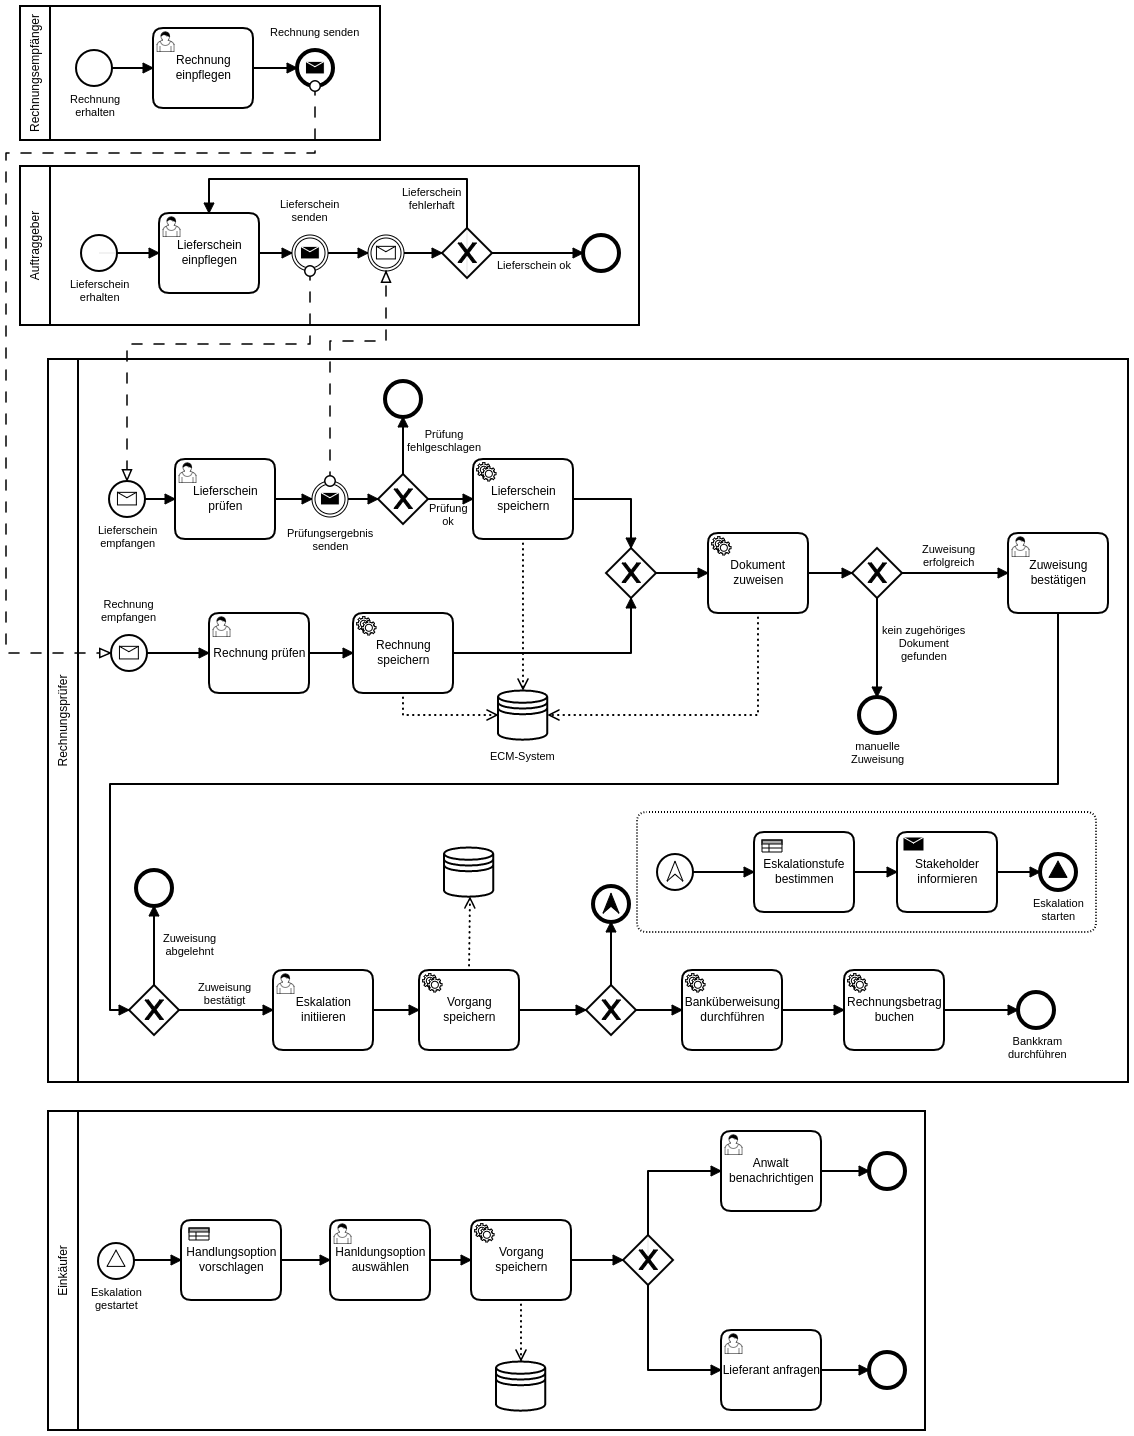
\includegraphics{images/rechnung.png}
  \caption{Bestellprozess}
  \label{fig:WF-Bestellprozess}
\end{figure}

\section{Verteilungssicht}\label{section-deployment-view}

Abbildung \ref{fig:Verteilungssicht} zeigt die Verteilungssicht für den selektierten Ausschnitt des Systems (ausgegraute Elemente sind nicht Teil des Prototypen). Die Rechnungsverwaltung, die Lieferscheinverwaltung, der Zuordnungsservice und die Finanzverwaltung sind eigenständige Java-Applikationen, die über HTTP/REST mit dem Server kommunizieren. Bei dem Server handelt es sich um eine embedded Tomcat Instanz, die von SpringBoot gestartet wird und die Camunda-Engine ausführt. Die Entscheidungstabellen und die BPM-Workflows können mit der Desktop-Anwendung Camunda Modeler entwickelt und über HTTP auf den Server deployed werden.

\begin{figure}
  \centering
  \includegraphics{images/Verteilungssicht.png}
  \caption{Verteilungssicht}
  \label{fig:Verteilungssicht}
\end{figure}

\section{Querschnittliche Konzepte}\label{section-concepts}

\subsection{Domänenmodell}

In Abbildung \ref{fig:geschaeftsobjekte} ist das Domänenmodell dargestellt.

\begin{figure}
  \centering
  \includegraphics{images/geschaeftsobjekte.png}
  \caption{Geschäftsobjekte}
  \label{fig:geschaeftsobjekte}
\end{figure}

\subsection{Skalierbarkeit}

\paragraph{Prinzip 1 - Klonen eines Services} Camunda bietet zwei varianten Service Tasks auszuführen, entweder als \textit{internal Service-Task} oder als \textit{external Serivce-Task}. Bei einem internal Service-Task wird eine Java-Klasse, die das Camunda Interface JavaDelegation implementiert, ein Objekt, eine Objekt-Methode oder ein Skript aufgerufen. Die Funktionalität wird mit der Applikation deployed. Anders ist es bei external Service-Tasks. Diese Tasks werden nicht aufgerufen, sondern holen sich eigenständig ihre Aufgaben über HTTP von der Applikation (\href{https://docs.camunda.org/manual/latest/user-guide/process-engine/external-tasks/}{https://docs.camunda.org/manual/latest/user-guide/process-engine/external-tasks/}). Bearbeitet ein external Service-Tasks eine Aufgabe, kann er die Aufgabe für andere Tasks sperren. Das erlaubt, dass jedem external Service-Tasks eine freie Aufgabe zugewiesen bekommt und das Skalieren, durch mehrfaches starten einer external Service-Tasks-Instanz bzw. Klonen, leicht möglich ist.

\paragraph{Prinzip 2 - Fachliche Aufteilung eines Services} Es wurden die Fachlichkeiten „Rechnung in System einpflegen“ bzw. „Rechnung versenden“ getrennt. Das Gleiche gilt für die Digitalisierung des Lieferscheins.

\paragraph{Prinzip 3 - Teilung eines Service nach Consumer-Typen} Die Services wurden nach Auftraggeber, Rechnungsempfänger, Rechnungsprüfer und Einkäufer getrennt.

\paragraph{Prinzip 4 - Teilung nach Read/Write} Das Lesen bzw. Finden von zusammengehörigen Rechnungen und Lieferscheinen und das Schreiben bzw. Speichern der Zuordnung wurde getrennt.

\paragraph{Prinzip 5 - CQRS} Die Umsetzung würde die Gesamtarchitektur komplexer machen. Ein Qualitätsziel des Prototypen war Verständlichkeit.

\paragraph{Prinzip 6 - Lokalisierung eines Service} Services können an einem beliebigen Ort deployed werden. Die Kommunikation wird über HTTP vollzogen.

\paragraph{Prinzip 7 - Bildung von Caches} Bisher werden keine Daten in eine Datenbank geschrieben, daher sind alle Daten nur lokal gespeichert bzw. „gecached“.

\paragraph{Kompensation}
\begin{itemize}
\item Rechnung falschem Lieferschein zugeordnet → Zuordnung rückgängig machen
\item Lieferschein kann keiner Rechnung zugeordnet werden → Zuordnung rückgängig machen
\item Fehler bei der Transaktion → Rückbuchung veranlassen
\end{itemize}

\section{Entwurfsentscheidungen}\label{section-design-decisions}

\subsection{Reports}

Im Prototyp werden keine Reports erstellt. Camunda enthält in der Enterprise-Edition Funktionen zum Erstellen von Reports. Alternativ könnten die Funktion durch Plug-ins oder zusätzliche Service Tasks realisiert werden.

\subsection{Deployment}

Camunda kann innerhalb von Spring Boot bzw. innerhalb des Spring Frameworks, über Docker oder „standalon“ z.B. in einem Tomcat-Server deployed werden. Für den Prototypen wurde entschieden, Camunda innerhalb einer Spring Boot-Anwendung zu deployen, da das Vorgehen neben Java keine Anforderungen an den Entwicklerrechner stellt. Für den Produktiveinsatz scheint die Verwendung von Docker die meiste Flexibilität (Verwendung eines Cloud-Dienstes oder On-Premise) zu bieten.

\subsection{Cloud vs. On-Premise}

Der Business-Case in Abbildung \ref{fig:business-case} zeigt, dass langfristig eine On-Premise Lösung zu bevorzugen ist.

\begin{figure}
  \centering
  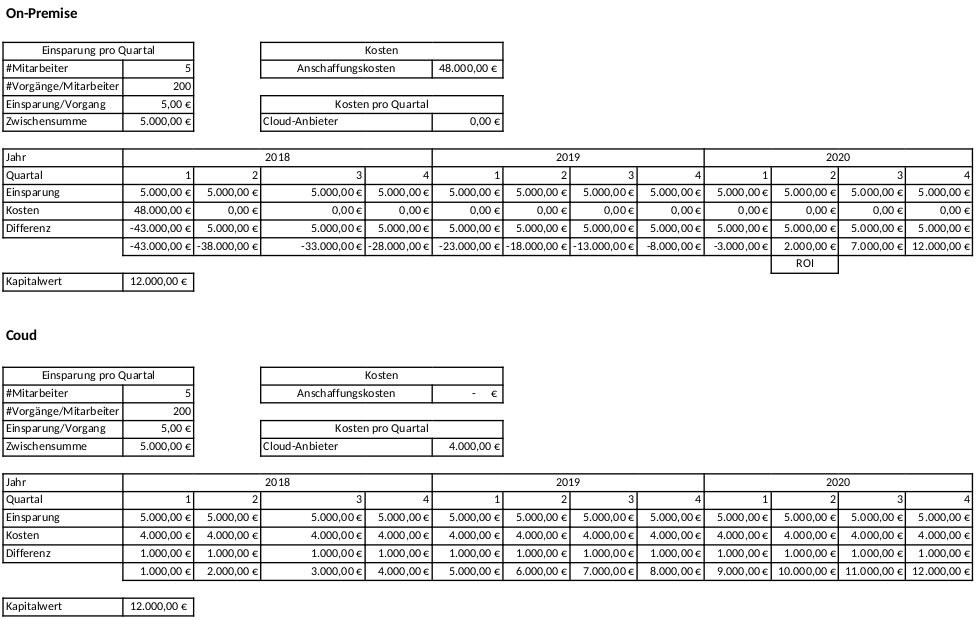
\includegraphics{images/business-case.png}
  \caption{Business Case}
  \label{fig:business-case}
\end{figure}

\subsection{Benutzereingabe}

Camunda bietet verschiedene Möglichkeiten, Formulare zu erstellen:
\begin{description}
  \item[Embedded Task Forms] HTML-Dokument definieren, welches innerhalb der Tasklist angezeigt wird.
  \item [Generated Task Forms] Formular innerhalb des Modellers mittels XML beschreiben.
  \item[External Task Forms] HTML-Dokument definieren, auf welches verlinkt wird.
  \item [Generic Tasks Forms] Der Anwender gibt Variablenname, Typ und Wert beim Starten eines Tasks an.
\end{description}

Für den Prototypen wurden Generated Task Forms verwendet, die Variante hat das beste Verhältnis zwischen Aufwand und Komfort geboten, um mit den BPM-Modell zu experimentieren.

\section{Risiken und technische Schulden}\label{section-technical-risks}

Das System ist aktuell stark von der Camunda-Plattform abhängig. Da die Camunda-Plattform bereits in verschiedenen Unternehmen erfolgreich produktiv eingesetzt wird, kann davon ausgegangen werden, dass die Plattform stabiler läuft als es eine Eigenentwicklung zu beginn tun würde. Dennoch stellt die Camunda-Plattform eine Möglichkeit für einen Single Point of Failure dar. Einzelne Komponenten, wie beispielsweise die Taskslist oder das Cockpit könnten ggf. nach und nach durch Eigenentwicklungen ausgetauscht werden.

Es werden zurzeit keine Reports erstellt. Die Enterprise-Edition von Camunda bietet die entsprechende Funktion, die Anschaffung könnte jedoch über dem Budget des Unternehmens liegen.

Die Taskslist entspricht nicht dem Corporate Design des Unternehmens. Außerdem wurde für den Prototypen von Camunda generierte Formulare verwendet. Für komplexe Eingaben ist evtl. die Verwendung eines anderen Formulartypen vorteilhafter. Die Taskslist und die Formulare könnten zum Beispiel mit Angular, React oder Vue.js erstellt werden, siehe den Eintrag im Camunda-Blog (\href{https://blog.camunda.com/post/2018/02/custom-tasklist-examples/}{https://blog.camunda.com/post/2018/02/custom-tasklist-examples/}).

BPM-Diagramme können schnell unübersichtlich werden, sobald neben dem „Happy-Path“ auch alle Ausnahmefälle modelliert werden. Dann ist vielleicht eine Aufteilung der Workflows auf verschiedenen Dateien nötig. Die Verwendung von zusätzlichen Elementen, wie beispielsweise Subprozessen, könnte ebenfalls helfen, die Übersicht zu verbessern.


\end{document}
